%% ==============================
\chapter{Results}
\label{sec:results}
%% ==============================
Questions to ask:
\begin{enumerate}
    \item What is the result of your work?
    \item What metrics do you use to measure the effect of your work?
    \item What are the parameters of your evaluation? (sample size, goal metric, different configurations)
    \item How do you compare to existing approaches?
    \item How does this result answer your research question?
\end{enumerate}

\begin{enumerate}
    \item Comparison of planners on rooms
    \item Advantages of ILIR in distortion of public space
    \item Proof of concept 
\end{enumerate}

The result of this work are the straight path planner ILIR, the hierarchical planning algorithm and the planner plugin for integration in ROS 2. In this chapter these approaches are evaluated and compared to related work. The criteria for evaluation were presented in Chapter \ref{sec:methods} "Methods".

%% ==============================
\section{Comparison of Straight Path Planners}
\label{sec:evaluation_straight_path}
%% ==============================
The evaluation of the planner algorithm ILIR is done on the benchmark maps from Ryu \cite{ryu_hierarchical_2020} and Hou \cite{hou_straight_2021}. And to specifically show the effects of the disturbance of public space, the second room of the first map and the ninth room of the second map were chosen. The metrics and the calculation of path numbers were presented in Chapter \ref{sec:methods} but for better readability a complete list is repeated here:

\begin{enumerate}
  \item \textbf{Success rate}: Percentage of valid paths found
  \item \textbf{Path length}: Total length from start to goal in pixels
  \item \textbf{Planning time}: Total time for planning including smoothing
  \item \textbf{Path smoothness}: Sum of deviation angles divided by path length
  \item \textbf{Obstacle clearance}: Mean distance from path to obstacles
  \item \textbf{Distance deviation}: Standard deviation of the distance between path and obstacle
  \item \textbf{Distance to centroid}: Mean distance from path to centroid of the room
  \item \textbf{Disturbance of public space}: Largest open area inside roadmap divided by total room area (Details in Chapter \ref{sec:new_metric})
\end{enumerate}

The different planner which are compared to the ILIR algorithm are listed below. These planners were chosen because they are widely used in the field of path planning for robotics and provide a good baseline to compare to. Additionally the A* can bee seen as a ground truth for the shortest path distance as it is complete and optimal. The other two represent a very different approach of probabilistic sampling.

\begin{enumerate}
    \item \textbf{ILIR}: Iterative Largest Interior Rectangle
    \item \textbf{A*}: A* Planner
    \item \textbf{PRM}: Probabilistic Roadmap
    \item \textbf{RRT}: Rapidly exploring Random Tree
\end{enumerate}

\begin{figure}[h]
    \captionsetup[subfigure]{justification=centering}
    \centering
    \begin{subfigure}{.25\textwidth}
      \centering
      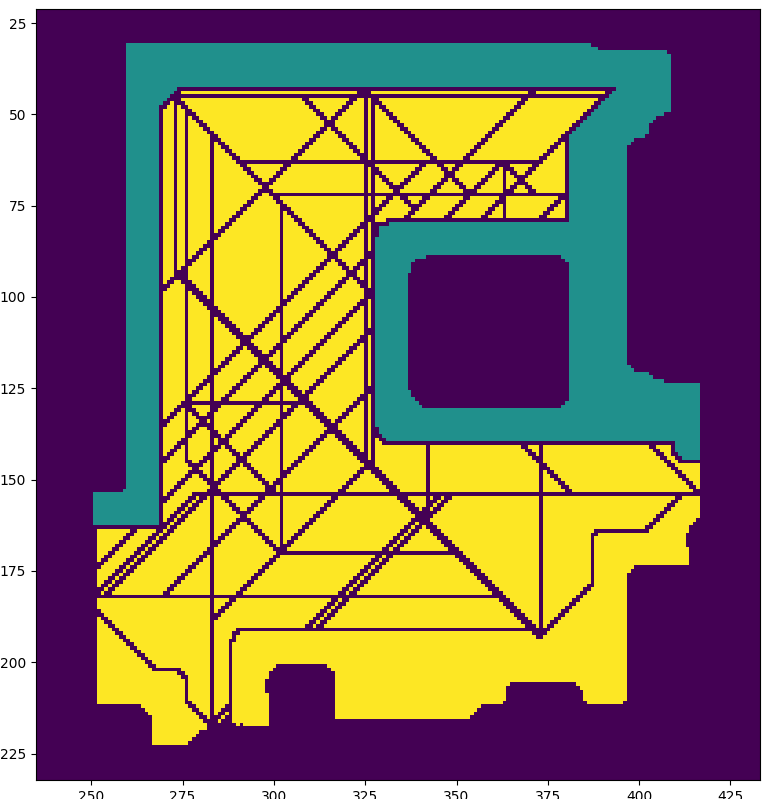
\includegraphics[width=\textwidth]{figures/60_results/room2_disturbance_astar_unsmoothed.png}
      \caption{A* Planner}
    \end{subfigure}%
    \begin{subfigure}{.24\textwidth}
      \centering
      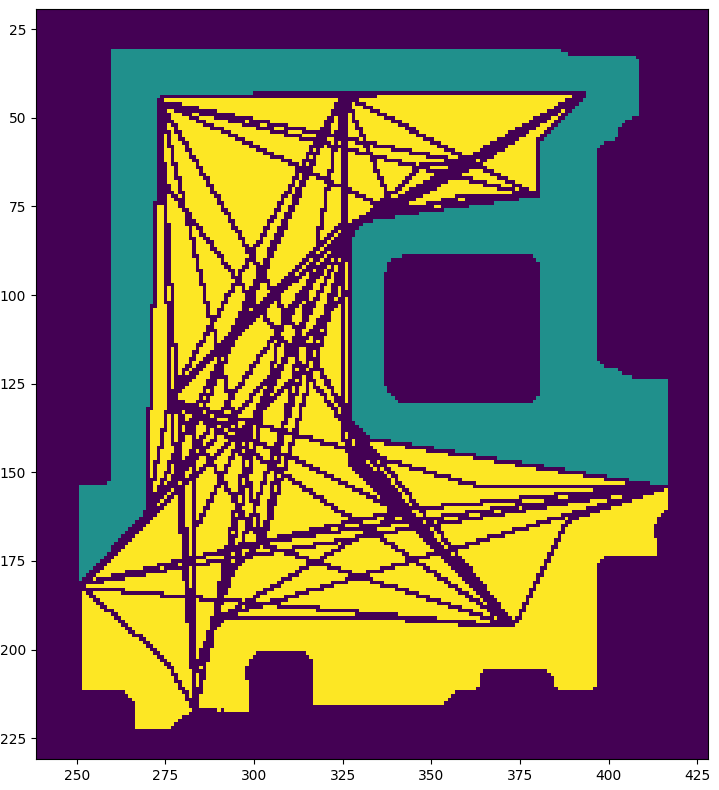
\includegraphics[width=\textwidth]{figures/60_results/room2_disturbance_astar_smooth.png}
      \caption{A* smoothed}
    \end{subfigure}
    \caption[Comparison of A* with and without smoothing algorithm]{Comparison of A* with and without smoothing algorithm. Turquoise and yellow areas are both representing the original room map.}
    \label{fig:smoothing}
\end{figure}

The first step for a fair comparison is to smooth the output path of each planner as it would realistically be used by a robot for driving. This is necessary because the A* for example produces paths on a gridmap which has a certain resolution. This leads to "steps" for diagonal lines. And there are always many possible solution paths which have the exact same path length. It is only determined by the order of node expansion by the specific implementation. To force the path to take the most direct route, unnecessary nodes are removed and the more direct connection is chosen. In Figure \ref{fig:smoothing} the effect of this smoothing can be seen. The same is done for the PRM and RRT. Both of these planners create a roadmap by sampling random points in the environment. This roadmap is then connected and provides a path. This is not optimal because there a many unnecessary turns. For smoothing the nodes with the highest deviation angles between the ingoing and outgoging line are tried to be removed. If this is possible, the surrounding nodes are connected directly and the process is repeated until no node can be removed anymore because it would otherwise result in a collision path. This is not done for the ILIR because this would counter the goal of leaving out the middle are for undisturbed human traffic.

\begin{figure}[h]
    \captionsetup[subfigure]{justification=centering}
    \centering
    \begin{subfigure}{.25\textwidth}
      \centering
      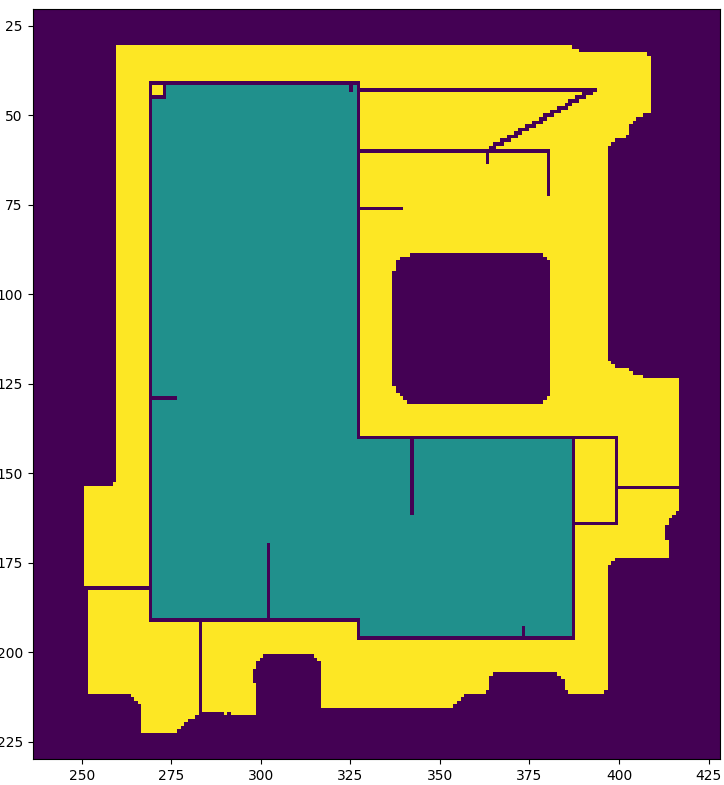
\includegraphics[width=\textwidth]{figures/60_results/room2_disturbance_ilir.png}
      \caption{ILIR}
    \end{subfigure}%
    \begin{subfigure}{.25\textwidth}
      \centering
      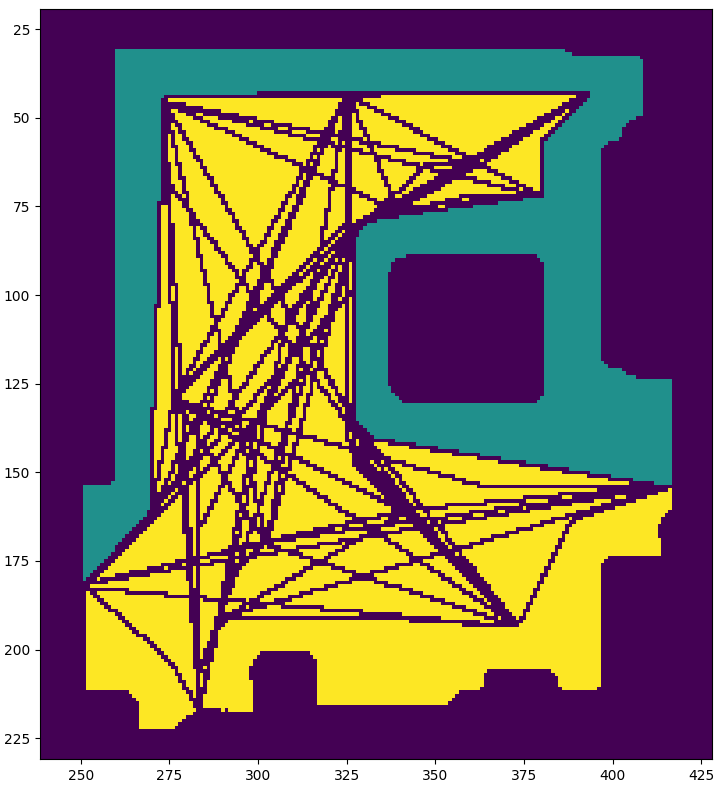
\includegraphics[width=\textwidth]{figures/60_results/room2_disturbance_astar.png}
      \caption{A*}
    \end{subfigure}%
    \begin{subfigure}{.25\textwidth}
      \centering
      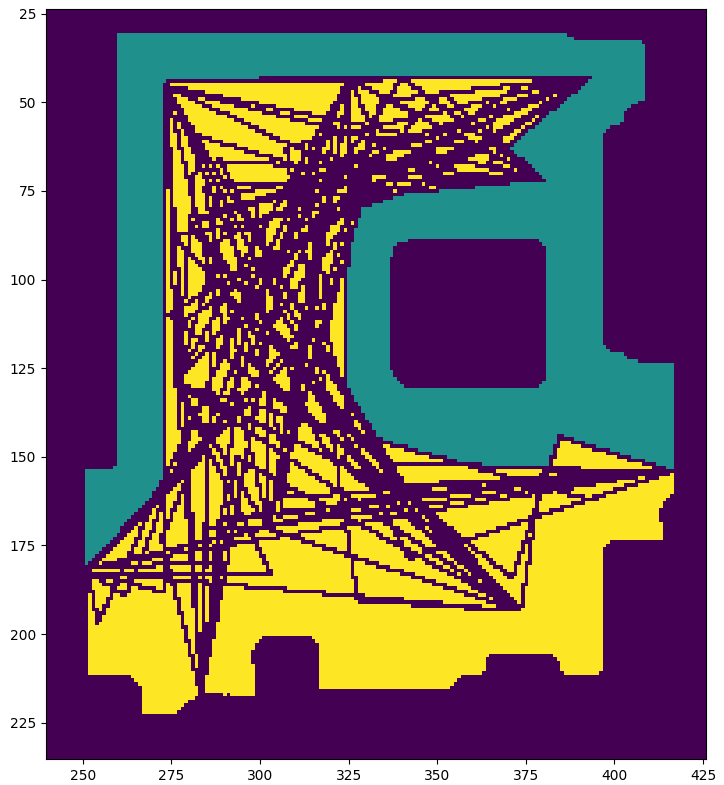
\includegraphics[width=\textwidth]{figures/60_results/room2_disturbance_prm.png}
      \caption{PRM}
    \end{subfigure}%
    \begin{subfigure}{.25\textwidth}
      \centering
      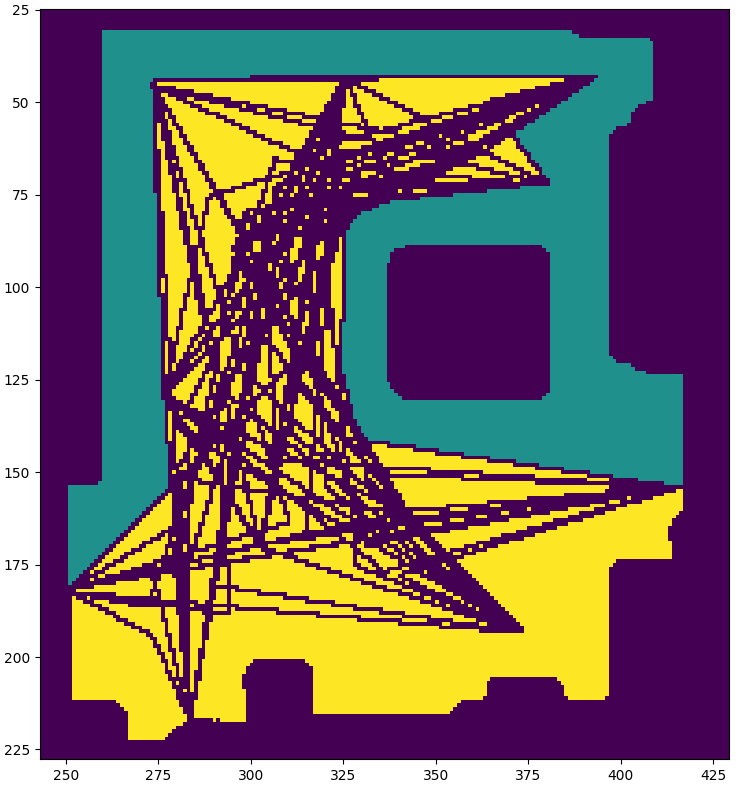
\includegraphics[width=\textwidth]{figures/60_results/room2_disturbance_rrt.png}
      \caption{RRT}
    \end{subfigure}
    \caption[Comparison of planning methods on room 2 of benchmark map 1 with 78 paths]{Comparison of planning methods on room 2 of benchmark map 1 with 78 paths. The turquoise area is the largest free area where no path is crossing and the combination with yellow is the original room map.}
    \label{fig:ryu_room2_comparison}
\end{figure}

In Figure \ref{fig:ryu_room2_comparison} the comparison of smoothed paths on the second room of the first benchmark map is shown. It can be clearly seen, that the ILIR planner forces the paths onto its roadmap and keeps clear of the inner area. In the graphics the metric for disturbance of public space is visually represented by the colors of the background. the turquoise area is the largest free area where no path is crossing and the remaining area is yellow. The calculation of this metric is explained in Chapter \ref{sec:methods} with the formula \ref{equ:disturbance}.

\todo{update ryu results with distance to centroid}
\begin{table}[ht]
\centering
\begin{tabular}{lc|cccc}
\hline
\textbf{Metric} & \textbf{Unit} & \textbf{ILIR} & \textbf{A*} & \textbf{PRM} & \textbf{RRT} \\
\hline
Success rate & - & 1.00 & 1.00 & 1.00 & 1.00 \\
Mean planning time & s & 0.17 & 1.04 & 0.93 & \textbf{0.02} \\
Mean path length & px & 187.92 & \textbf{119.11} & 137.62 & 132.60 \\
Mean smoothness & °/px & 2.37 & \textbf{0.29} & 0.39 & 0.36 \\
Mean obstacle clearance & px & \textbf{16.74} & 22.62 & 25.62 & 25.51 \\
Obstacle clearance std & px & \textbf{3.28} & 4.80 & 4.30 & 4.39 \\
Mean distance to centroid & px & - & - & - & - \\
Disturbance of public space & - & \textbf{0.53} & 0.70 & 0.67 & 0.67 \\
\hline
\end{tabular}
\caption{Comparison of planning methods on room 2 of benchmark map 1 with 78 paths}
\label{tab:room2_results}
\end{table}

In Table \ref{tab:room2_results} the results of the evaluation can be seen for each planner. The room 2 represents an average room which could appear on most floor in a office environment. It is only about ~8x6 m large. But already in this small room, the differences between the planners are visible. Due to its probabalistic nature and early check for a valid path before the complete roadmap is built, the RRT is the fastest with 0,02 s followed directly by ILIR with 0,17 s. In terms of path lenght, as expected, the A* Planner gives the shortest path and ILIR has the longest as it leaves out the middle area. The smoothness is a factor which is surprisingly bad for the ILIR with 2,37 °/px. It was expected, that with forcing straight paths the resulting path would be smoother. But this is a deceptive conclusion as it has more 90° turns than the others. This sums up to a large total turn angle and can not be compensated through the longer path. The obstacle clearance of ILIR is low which is not necessarily a bad thing as it shows that the paths are more closer to the wall. With the standard deviation of this distance it can be shown that these paths are also more consistent than the others. The metric of the distance to the centroid of the room also shows that the paths of ILIR are not going directly through the middel. This means the paths are close to the walls and generally less fluctuating than the paths from the other planners. Finally the custom metric for the disturbance of the room space shows that ILIR has the lowest disturbance with 0.53. This proves that the ILIR planner achieves its goal of planning paths that are straight and do not disturb the human working area even in a small room. Also in the Figure \ref{fig:ryu_room2_comparison} it can be well seen that the paths are deterministic and always follow the same roadmap. This makes them more predictable for human.

\begin{figure}[h]
    \captionsetup[subfigure]{justification=centering}
    \centering
    \begin{subfigure}{.35\textwidth}
      \centering
      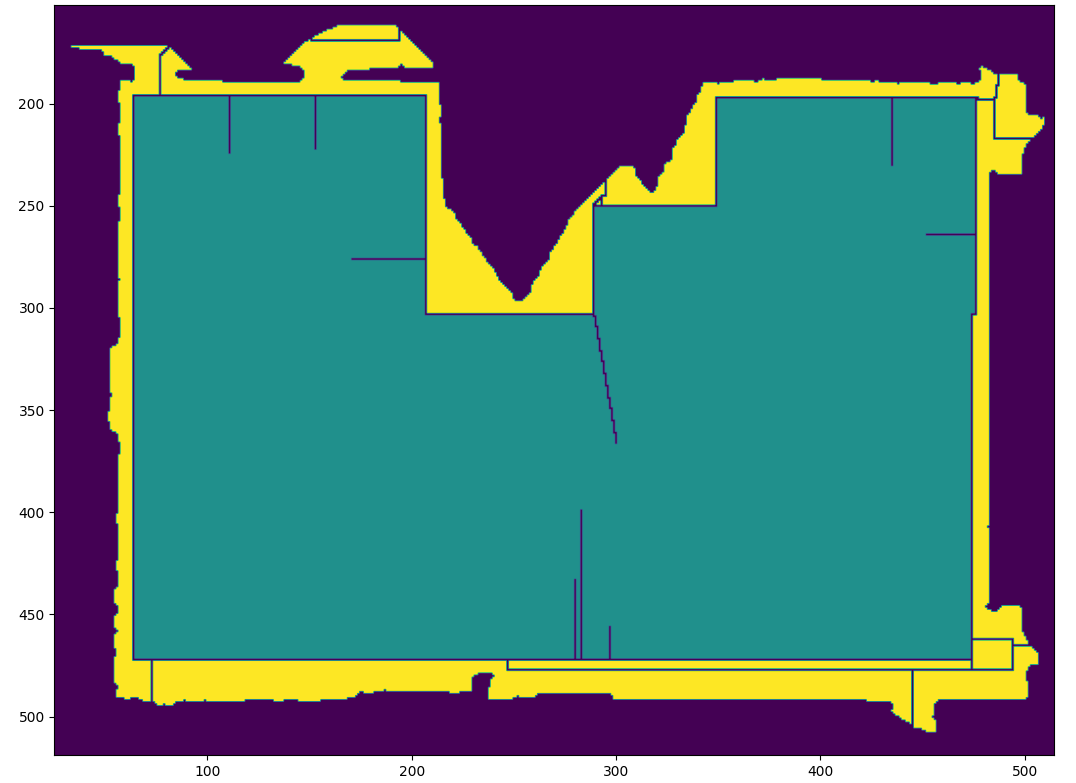
\includegraphics[width=\textwidth]{figures/60_results/room9_disturbance_ilir.png}
      \caption{ILIR}
    \end{subfigure}%
    \begin{subfigure}{.35\textwidth}
      \centering
      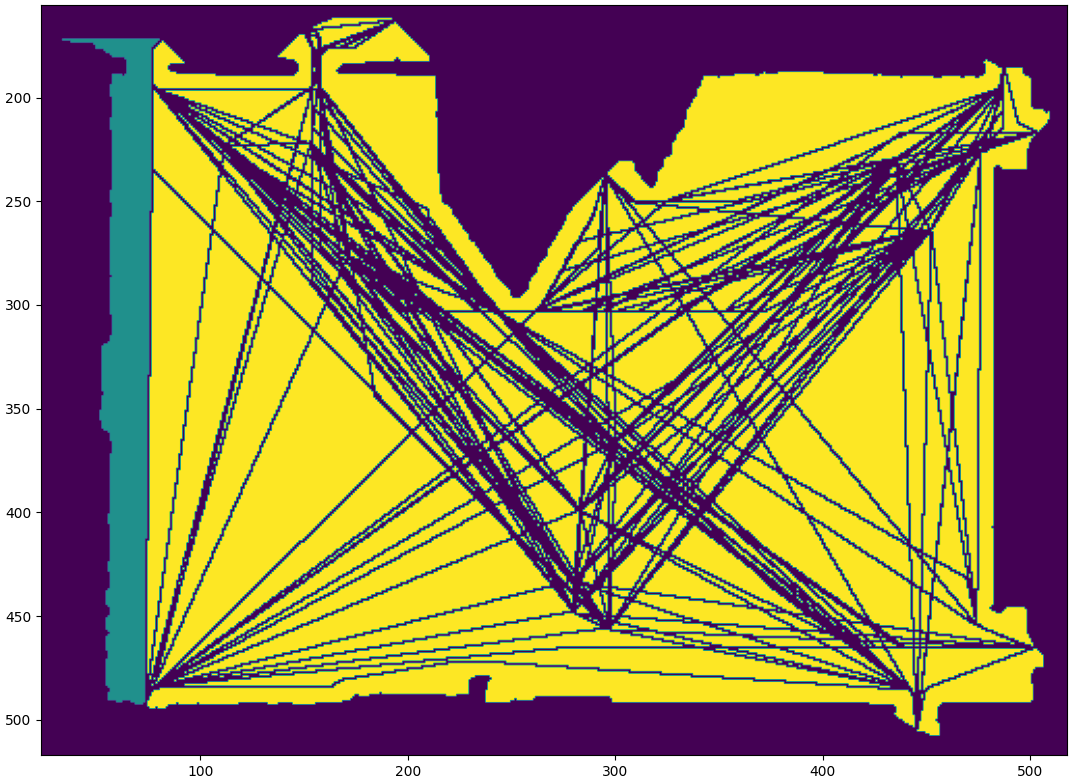
\includegraphics[width=\textwidth]{figures/60_results/room9_disturbance_astar.png}
      \caption{A*}
    \end{subfigure}
    \begin{subfigure}{.35\textwidth}
      \centering
      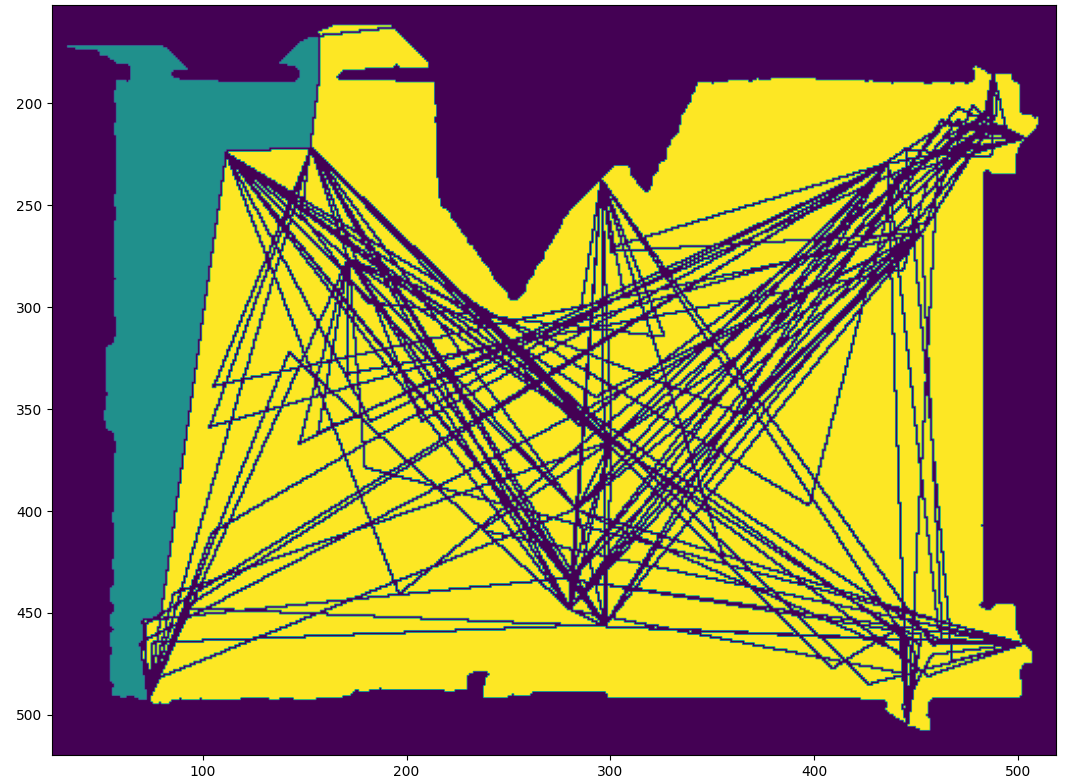
\includegraphics[width=\textwidth]{figures/60_results/room9_disturbance_prm.png}
      \caption{PRM}
    \end{subfigure}%
    \begin{subfigure}{.35\textwidth}
      \centering
      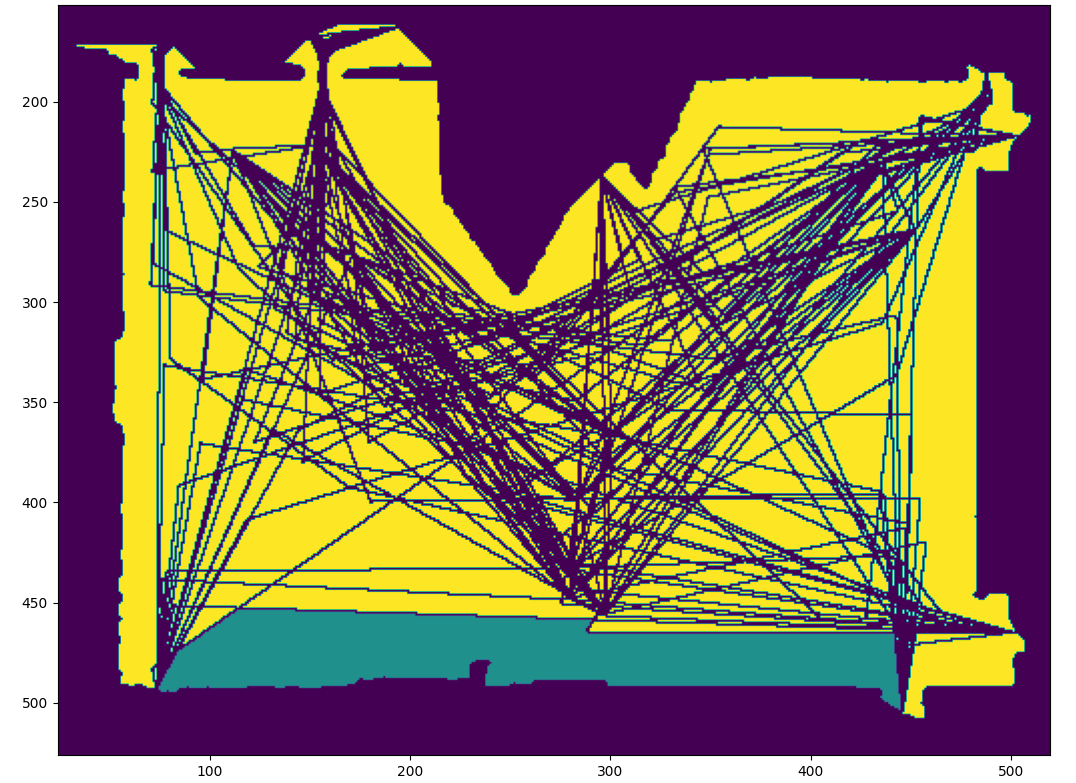
\includegraphics[width=\textwidth]{figures/60_results/room9_disturbance_rrt.png}
      \caption{RRT}
    \end{subfigure}
    \caption[Comparison of planning methods on room 9 of benchmark map 2 with 171 paths]{Comparison of planning methods on room 9 of benchmark map 2 with 171 paths. The turquoise area is the largest free area where no path is crossing and the combination with yellow is the original room map.}
    \label{fig:hou_room9_comparison}
\end{figure}

\todo{update hou2 results with distance to centroid}
\begin{table}[h]
\centering
\caption{Planner Metrics}
\label{tab:room9_results}
\begin{tabular}{lc|cccc}
\hline
\textbf{Metric}                    & \textbf{Unit} & \textbf{ILIR} & \textbf{AStar} & \textbf{PRM} & \textbf{RRT} \\
\hline
Success Rate                       & -             & 0.80          & \textbf{1.00}           & 0.63         & 0.95         \\
Planning Time                      & s             & \textbf{0.22}          & 8.09           & 0.95         & 0.78         \\
Mean Path Length                   & px            & 471.56        & 265.56         & \textbf{261.26}       & 300.90       \\
Mean Smoothness                    & °/px          & 1.22          & 0.26           & \textbf{0.19}         & 0.26         \\
Mean Obstacle Clearance            & px            & \textbf{17.55}        & 44.85          & 54.01        & 52.39        \\
Obstacle Clearance Std Dev         & px            & \textbf{6.60}          & 19.81          & 17.83        & 16.01        \\
Mean Distance to Centroid          & px            & -             & -              & -            & -            \\
Disturbance of Public Space        & -             & \textbf{0.20}          & 0.95           & 0.89         & 0.91         \\
\hline
\end{tabular}
\caption{Comparison of planning methods on room 9 of benchmark map 2 with 171 paths}
\end{table}

For comparison these same metrics are now applied to a conference lobby which is much larger (~30x50 m) and has more entrances. In Figure \ref{fig:hou_room9_comparison} this room is shown. The corresponding result of the evaluation is displayed in Table \ref{tab:room9_results}. In this case the ILIR planner is even the fastest in terms of planning time with 0,22 s per path. The mean obstacle clearance, its standard deviation and the distance to the centroid show again that the paths of ILIR are closer to the walls and less fluctuating. The difference in disturbance of public space is even bigger and with only 20 percent of the room area occupied by potential paths of the robot it leaves enough space for human activities. 

In the previous evaluation some rooms were highlighted to demonstrate the capabilities of the planners on an average map as well as for an extreme case. But of course most distances the robot is driving are through corridors. Especially there the goal property of straight paths are important to avoid collisions with humans and to establish a predictable behavior. For this reason the focus of the following evaluation is on the straight paths and general appearance and not on the path-specific metrics. 

\todo{update hou2 roadmap}
\begin{figure}[h]
    \captionsetup[subfigure]{justification=centering}
    \centering
    \begin{subfigure}{.5\textwidth}
      \centering
      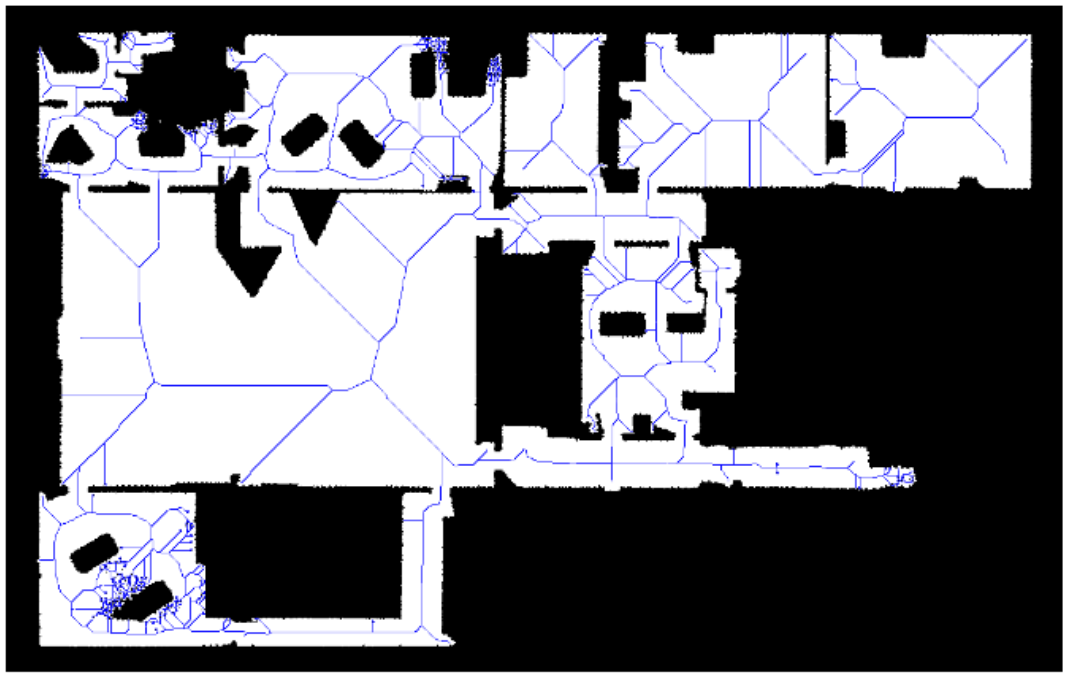
\includegraphics[width=\textwidth]{figures/60_results/hou2_roadmap_RGVG.png}
      \caption{RGVG}
    \end{subfigure}%
    \begin{subfigure}{.5\textwidth}
      \centering
      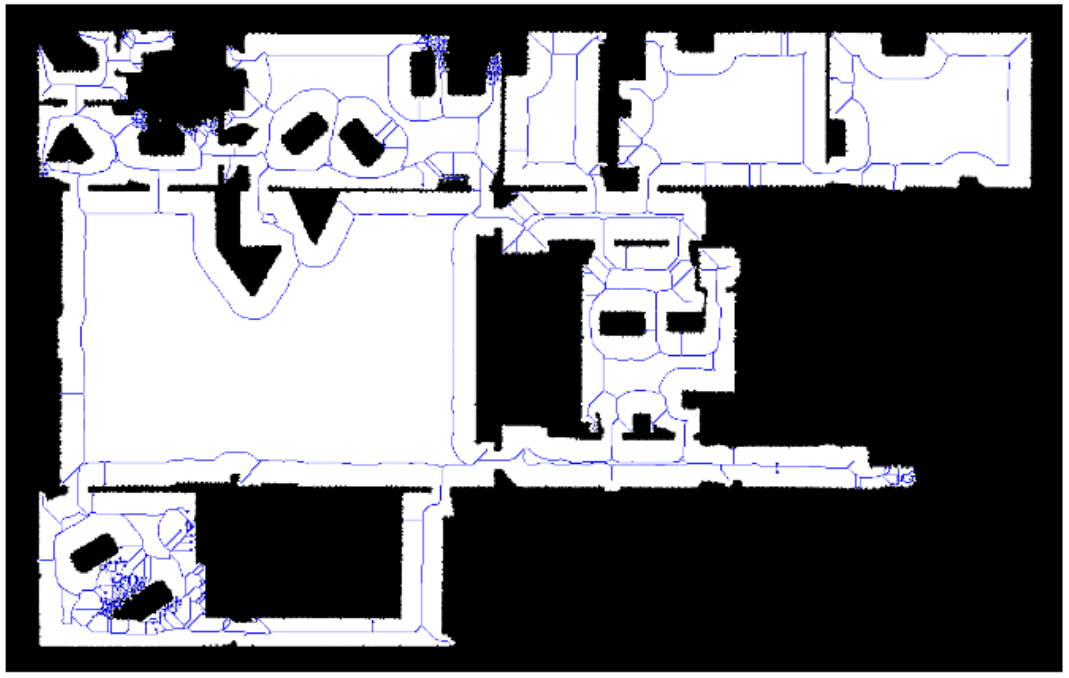
\includegraphics[width=\textwidth]{figures/60_results/hou2_roadmap_evg.png}
      \caption{EVG}
    \end{subfigure}
    \begin{subfigure}{.5\textwidth}
      \centering
      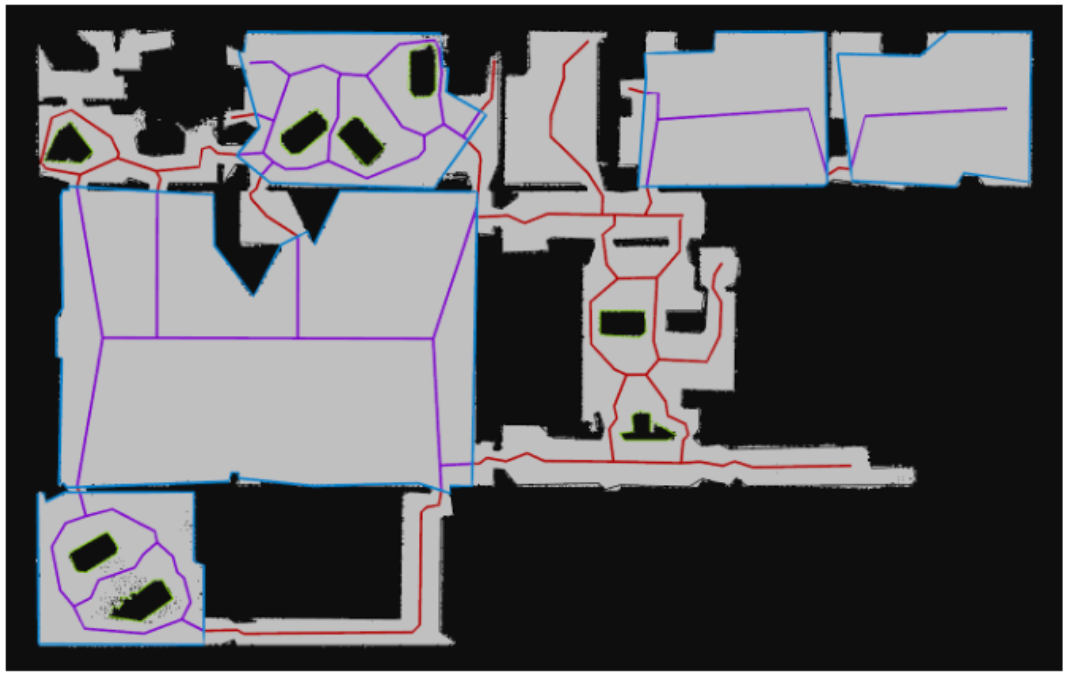
\includegraphics[width=\textwidth]{figures/60_results/hou2_roadmap_htm.png}
      \caption{HTM}
    \end{subfigure}%
    \begin{subfigure}{.5\textwidth}
      \centering
      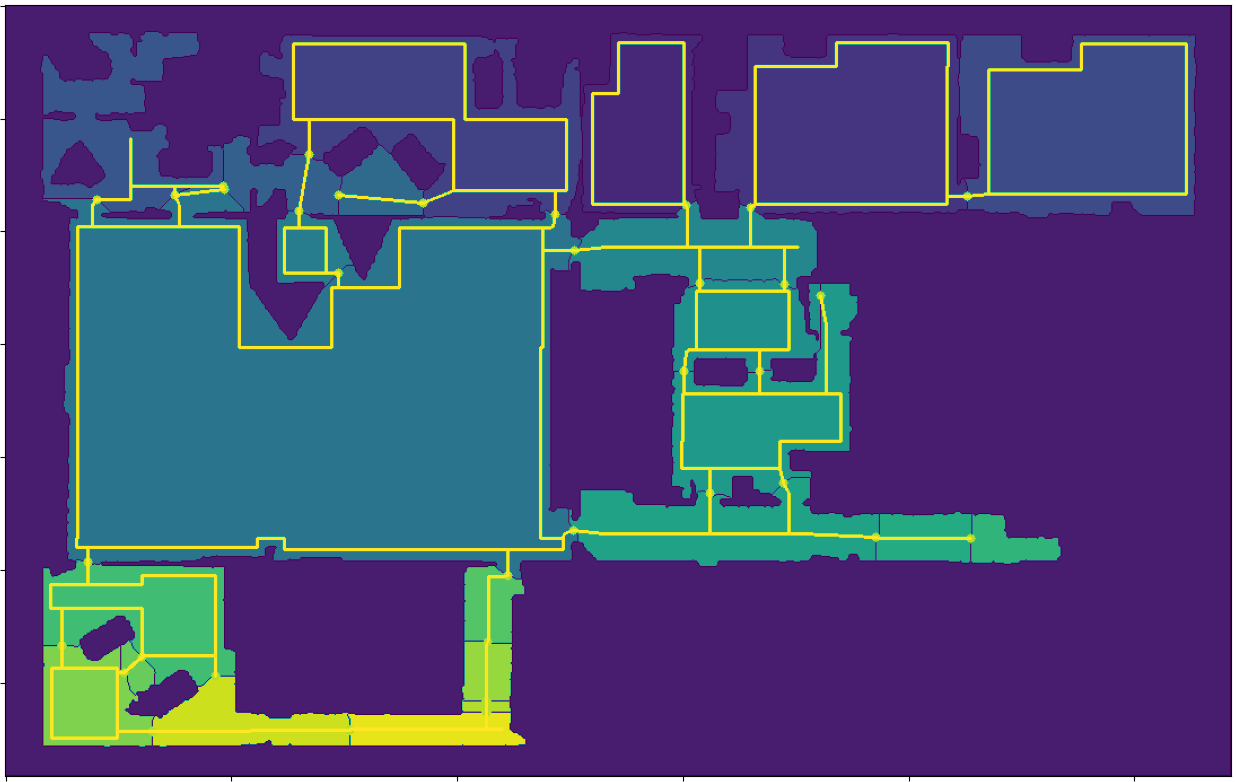
\includegraphics[width=\textwidth]{figures/60_results/hou2_roadmap_ilir.png}
      \caption{ILIR}
    \end{subfigure}
    \caption[Comparison of planning methods on room 9 of benchmark map 2 with 171 paths]{Comparison of planning methods on room 9 of benchmark map 2 with 171 paths. The turquoise area is the largest free area where no path is crossing and the combination with yellow is the original room map.}
    \label{fig:hou_comparison}
\end{figure}

In Figure \ref{fig:hou_comparison} the complete benchmark map 2 is shown and the roadmaps produced by the Reduced General Voronoi Graph (RGVG), the  Extended Voronoi Graph (EVG) \cite{beeson_towards_2005}, the Hierarchical Topological Map (HTM) \cite{hou_straight_2021} and the ILIR (this work) Planners. It can be seen, that the EVG in \ref{fig:hou_comparison} (b) is configured with a sensory horizon of 1.5 m, it always keeps close to the wall if there is a larger space. If not, it stay in the middle of the corridor. However it suffers from strong jiggle induced by sensor noise. The paths in the corridor are not straight and not good for driving with a robot. The HTM approach (c) solves the straight path problem for the corridor well but struggles in larger rooms. The paths are straight but almost never parallel to the walls and go straight through the open space. The ILIR planner (d) solves both of these problems by providing straight paths in the middle of each corridor while keeping close and parallel to the walls in large open areas. As the implementation of te other approaches are not open source it was not possible to directly compare these paths with specific metrics.

%% ==============================
\section{Comparison of Hierarchical Planners}
\label{sec:evaluation_hierarchical}
%% ==============================
The hierarchical planner has to be compared with other implementations from related work and on a set of benchmark that is comparable. As no such common set of benchmarks exist and the planners from related work are not open-source, this evaluation is only done as a proof-of-concept. However the SIRRT* algorithm from Ryu \cite{ryu_hierarchical_2020} uses the same benchmark map 1 and also implements a hierarchical planner. In Figure \ref{} a comparison between SIRRT* and the proposed hierarchical planner combined with the roadmap from ILIR can be seen. Note that the SIRRT* planner is limited to two levels of hierarchy as its focus is only in improving the calculation speed for paths in huge floors. 

\todo{Figure for ryu path from 10 to 7 compared with ilir path same rooms}

The proposed hierarchical planner (b) uses the H-Graph to efficiently plan first on room level and then only searches the corresponding roadmaps of these rooms. As these roadmaps can be precalculated a new search can be done very quickly. In comparison, the SIRRT* does an RRT search on each room for every path. This could also be sped up by caching the roadmap but is not described in \cite{ryu_hierarchical_2020}. The problem of choosing the correct room door for connections where two or more doors lead to the same room, is solved by both planners. This can be seen in (a) between room 16 and room 10. As well as in (b) on the same rooms. The shortest path inside room 16 would be to connect to the first door on the left but this would lead to an overall longer path. 

To further test the capabilities of the proposed hierarchical planner, a model of the research campus of \gls{iras} is created. It can be verified that the hierarchical planner is capable of planning between arbitrary paths in this complex environment. The H-Graph built has 4 hierarchy levels and total of \todo{XXX} nodes, the exact number on each hierarchy level can be seen in Table \ref{tab:ltc_graph_nodes}.

\todo{update number of nodes in graph}
\begin{table}[ht]
\centering
\begin{tabular}{lcc}
\hline
\textbf{Level} & \textbf{Name} & \textbf{Number of nodes} \\
\hline
Success rate & - & 1.00 \\
Mean planning time & s & 0.17\\
Mean path length & px & 187.92  \\
Mean smoothness & °/px & 2.37  \\
Mean obstacle clearance & px & \textbf{16.74}  \\
Obstacle clearance std & px & \textbf{3.28} \\
Mean distance to centroid & px & - \\
Disturbance of public space & - & \textbf{0.53} \\
\hline
\end{tabular}
\caption{Comparison of planning methods on room 2 of benchmark map 1 with 78 paths}
\label{tab:ltc_graph_nodes}
\end{table}

%% ==============================
\section{Evaluation in Simulation}
\label{sec:evaluation_simulation}
%% ==============================
To validate the developed concept, it is tested in a simulated hospital environment. The environment was previously presented in Figure \ref{fig:aws_hospital} in Chapter \ref{sec:simulation}. Amazon made their "AWS RoboMaker Hospital World" \cite{aws_robotics_aws_2023} open-source available but did not publish any research done with it. This means it was not possible to compare this approach with with related work in the area of multi-floor navigation on the same environment. However there is one work from Fredriksson et al. \cite{fredriksson_semantic_2023} which uses the same hospital simulation from Amazon but focus on detecting semantic features like intersections and corridors. It has also the aim of providing a clean roadmap for global navigation of the robot. In Figure \ref{fig:aws_comparison} a comparison of this approach and the resulting roadmap with the proposed planner and other related work like EVG and RGVG is shown.

\todo{update aws ilir roadmap}
\begin{figure}[h]
    \captionsetup[subfigure]{justification=centering}
    \centering
    \begin{subfigure}{.5\textwidth}
      \centering
      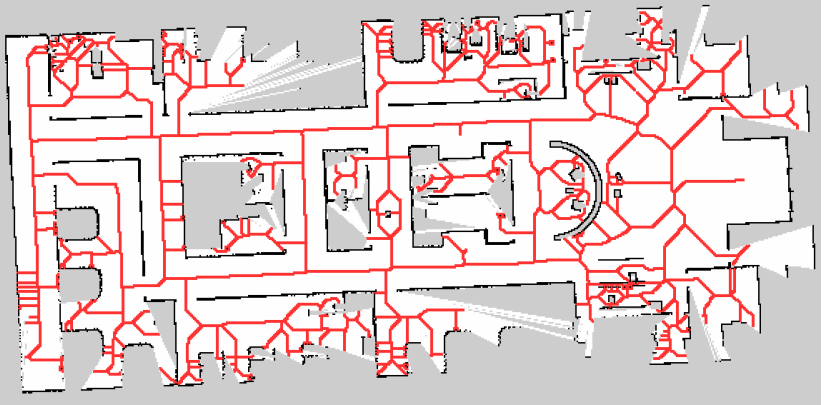
\includegraphics[width=\textwidth]{figures/60_results/aws_roadmap_rgvg.png}
      \caption{RGVG}
    \end{subfigure}%
    \begin{subfigure}{.5\textwidth}
      \centering
      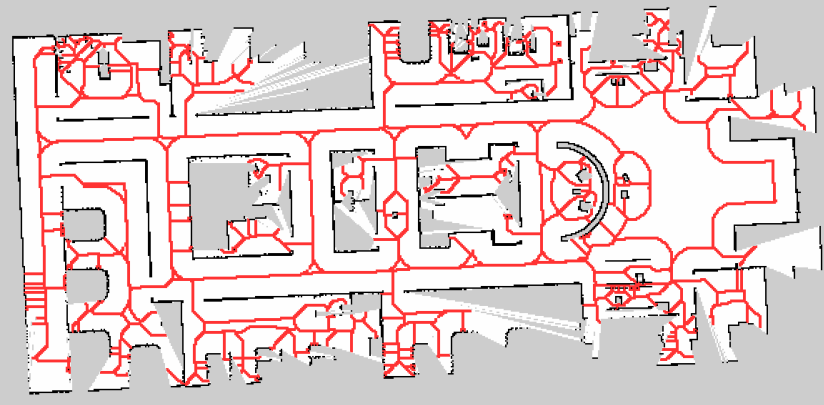
\includegraphics[width=\textwidth]{figures/60_results/aws_roadmap_evg.png}
      \caption{EVG}
    \end{subfigure}
    \begin{subfigure}{.5\textwidth}
      \centering
      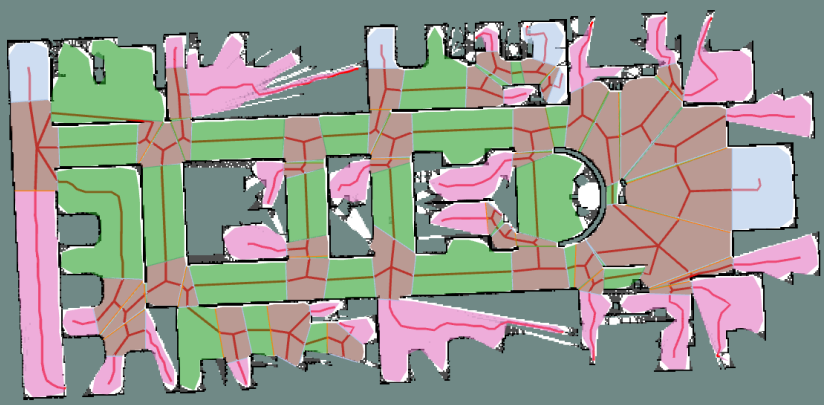
\includegraphics[width=\textwidth]{figures/60_results/aws_roadmap_semantic.png}
      \caption{Semantic \cite{fredriksson_semantic_2023}}
    \end{subfigure}%
    \begin{subfigure}{.5\textwidth}
      \centering
      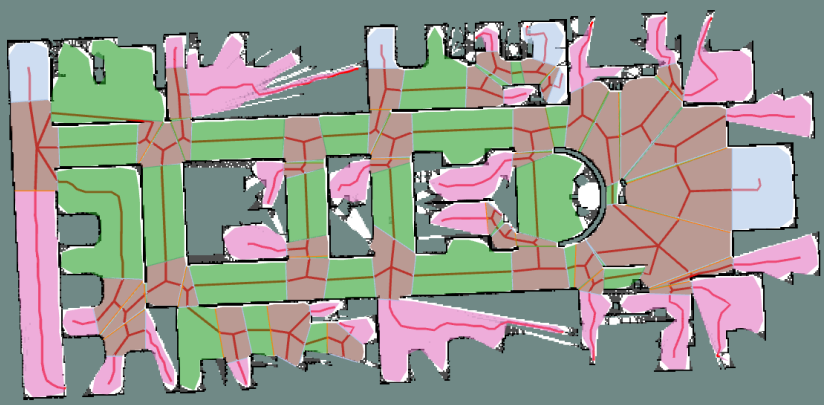
\includegraphics[width=\textwidth]{figures/60_results/aws_roadmap_semantic.png}
      \caption{ILIR}
    \end{subfigure}
    \caption[Comparison of planning methods for the hospital simulation]{Comparison of planning methods for the hospital simulation. For (c) semantic features are colored: Green for pathways, brown for intersections, blue dead ends and pink paths to a new frontier. In (d) the segmented rooms are colored with an increasing color palette, the roadmap is yellow.}
    \label{fig:aws_comparison}
\end{figure}

With this roadmap generated by ILIR \ref{fig:aws_comparison} (d), the complete multi-floor navigation with ROS 2 can be tested. Note that the simulation environment has two floors but they are duplicates of each other with the same layout. In Figure \ref{fig:aws_neobotix_simulation} the \gls{rviz} (left) and the Gazebo simulation (right) is shown. RVIZ represents all the data the robot knows about the environment. It doesnt matter for the robot if this data comes from a simulation or from sensors in the real world. The robot used in this simulation is the MPO\_500 from Neobotix because the same planners are used in the PeTRA project. The robot can be seen in RVIZ as well as in the bottom floor (the ceiling is transparent) on the left side. It emits blue rays from the laser scanner just for visualization. THe goal of this proof-of-concept is the elevator on the left side. In RVIZ the path from the hierarchiccal planner on the ILIR roadmap can be seen in as thin red line. There is also a smaller blue line which represents the current motion of the controller thath keeps the robot on the path. This is also used for smoothly drive around the sharp corners in the red roadmap. The goal given by the hierarchical planner is determined by the H-Graph as the shortest connection from the bottom floor to the upper floor. THe location of the elevators in the map was previously marked during graph creation. Once the robot reaches the elevator it will be teleported in simulation to the top floor and will get a new path to the final goal on the top floor. Once the final goal is reached another multi-floor navigation with its own behavior tree is triggered to bring the robot down on the bottom floor again. This behavior was successfully tested in a loop 10 times. This proves the capability of the developed multi-floor navigation system. 

\begin{figure}[h]
    \centering
    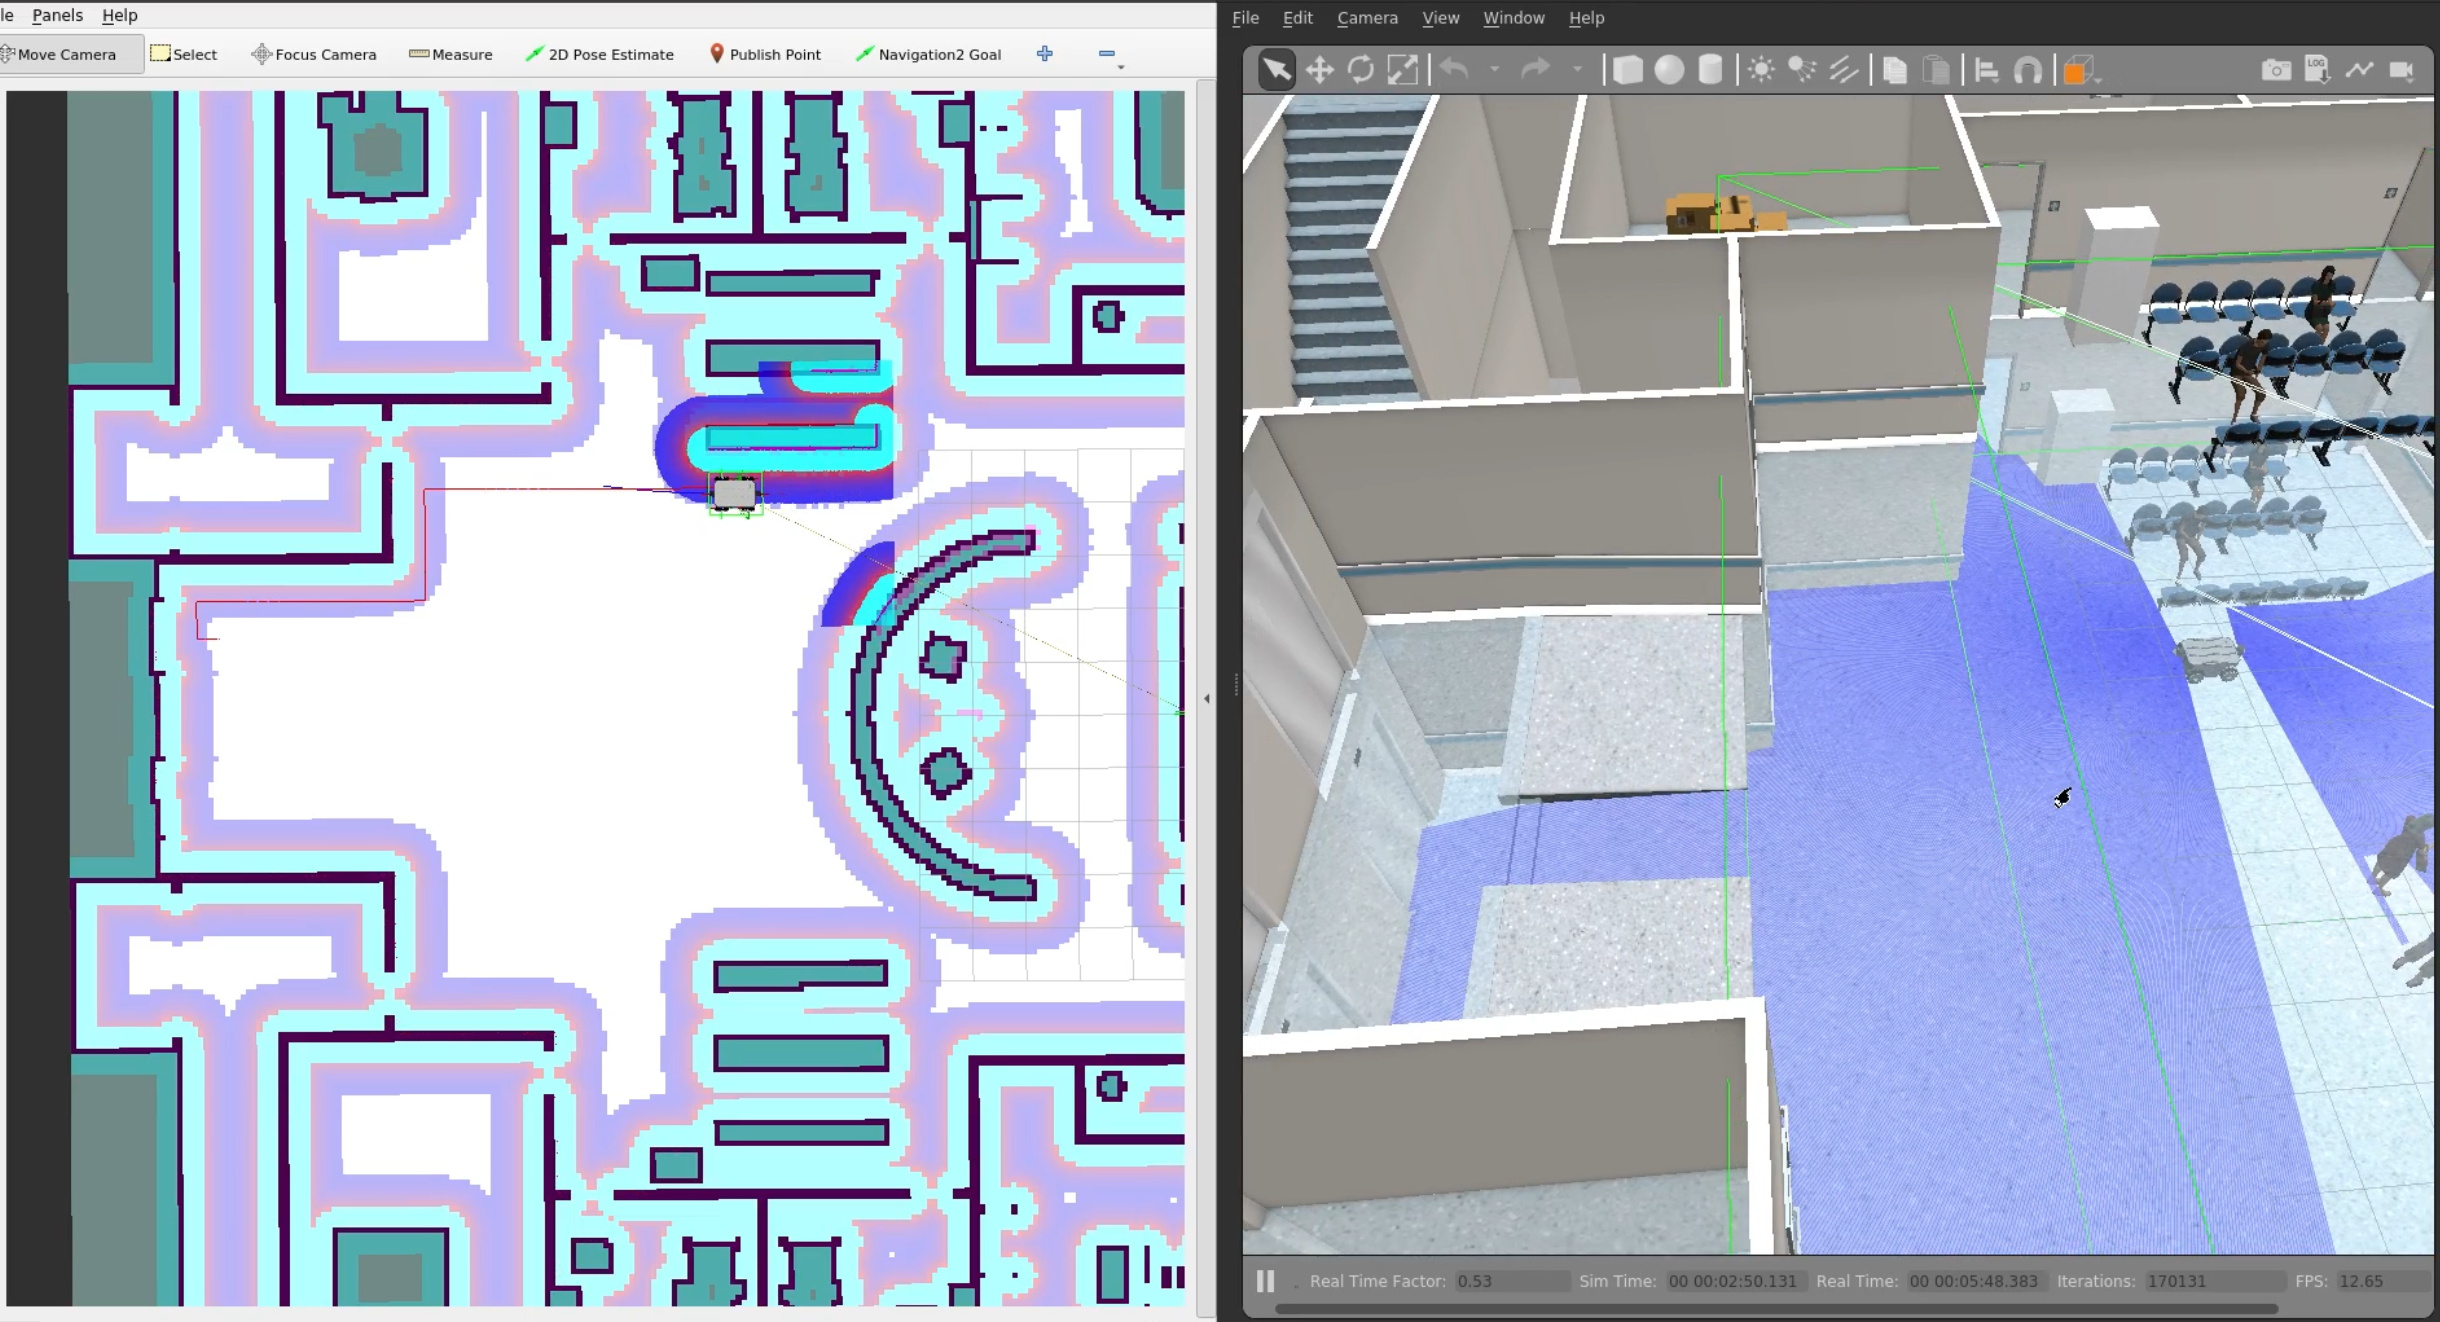
\includegraphics[width=\textwidth]{figures/60_results/aws_neobotix_simulation.png}
    \caption[UML diagram of the H-Graph implementation]{UML diagram of the H-Graph implementation. Blue components were taken from the community, green components were developed in this work.}
    \label{fig:aws_neobotix_simulation}
\end{figure}
